\documentclass[]{report}
\usepackage{amsmath}
\usepackage[framed,numbered,autolinebreaks,useliterate]{mcode}
\usepackage{graphicx}
\usepackage[parfill]{parskip}


\begin{document}

\section*{Results}
%---------------------------
% Q5
%---------------------------
\textbf{1. (i)} The decoded sentence is
$$
'thensaiswatchingyou'\, --> \, 'the\,nsa\,is\,watching\,you'
$$

\begin{figure}
\centering
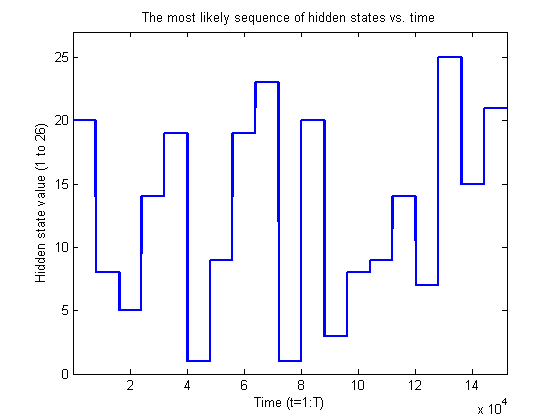
\includegraphics[scale=0.7, natwidth=305,natheight=380]{q1.png}
\caption{The most likely sequence of hidden states vs. time \label{fig:f1}}
\end{figure}

\begin{lstlisting} [caption=The MATLAB code for HMM speech recognizer  \label{listing:l1}]
%{
Author: Mehmet Koc
Description: HMM Speech Recognition
%}
close all
clear
%read data
Ot = importdata('observations.txt') + 1';
A = importdata('transitionMatrix.txt');
B = importdata('emissionMatrix.txt');
pi = importdata('initialStateDistribution.txt');
%%
T = length(Ot);
n = length(pi);
%compute max log-likelihood for all t=1:T
%also save the most probable state transitions
L = zeros(n, T);
phi = zeros(n, T);
l1 = log(pi) + log(B(:, Ot(1)));
L(:, 1) = l1;
for i = 2:T
    lMat = repmat(L(:, i-1), [1, n]); 
    [maxL, ind] = max(lMat + log(A));
    L(:, i) = maxL' +  log(B(:, Ot(i)));
    phi(:, i) = ind';
end
%%
%best state sequence
S = zeros(T, 1);
[~, S(T)] = max(L(:, T));
%backtracking
for i = (T-1):-1:1
    S(i) = phi(S(i+1), i+1);
end
isRepeated = false(T, 1);
for i = 2:T
   if(S(i) == S(i-1))
       isRepeated(i) = 1;
   end
end
%decode and eliminate repetitions
sentence = S(~isRepeated);
alphabet = char(97:122);
sentenceDecoded = alphabet(sentence);
%%
%plot the most likely sequence of hidden states vs time
figure, plot(S, 'linewidth', 2);
xlim([1, T]); ylim([0, n+1]);
xlabel('Time (t=1:T)'); ylabel('Hidden state value (1 to 26)');
title('The most likely sequence of hidden states vs. time');
\end{lstlisting}



\end{document}          
